\chapter[INTRODUÇÃO]{INTRODUÇÃO}
%---------------------------------------------------------------------------------------

A simulação numérica de problemas na engenharia possui uma grande importância tanto para o meio acadêmico quanto para a indústria favorecendo o desenvolvimento de novas tecnologias. Dado esse interesse, novas técnicas para aumentar a acurácia das simulações numéricas são de grande importância.

Esse trabalho verifica o erro de discretização que ocorre nas soluções do FVM usando-se uma malha não estruturada triangular comparando a solução com a analítica e suavizando a malha com vários algoritmos diferentes.
\criarsigla{FVM}{Método dos Volumes Finitos}

Muitos problemas de engenharia estão relacionados a geometrias complexas, em que o uso de um sistema de coordenadas cartesianas, cilíndricas ou esféricas não se mostra prático ou adequado. No cálculo numérico do fluxo sobre um semi cilindro, conforme a figura \ref{fig:semicilindro} temos que a fronteira da figura não coincide com as linhas coordenadas da malha estruturada, de modo que essa malha não é adequada para esse problema. \cite{Versteeg2007}

\begin{figure}[]
    \centering
    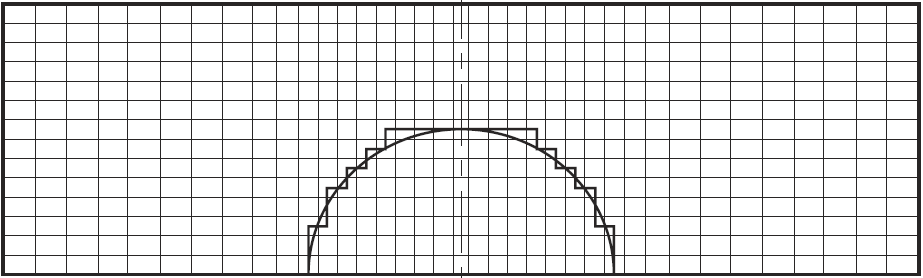
\includegraphics[width=.6\linewidth]{fig/semicilindro.png}
    \caption{Grade cartesiana para prever o fluxo em um semi cilindro}
    \label{fig:semicilindro}
\end{figure}

Malhas cartesianas são exemplos de um método estruturado. Como características de uma malha estruturada, tem-se:

\begin{itemize}
    \item os pontos nodais são posicionados nas interseções das linhas coordenadas.
    \item os pontos nodais interiores (que não estão posicionados nos contornos) possuem um número fixo de pontos nodais vizinhos.
    \item os pontos nodais podem ser mapeados dentro de uma matriz, sua localização na malha e na matriz é fornecida por índices (comumente i,j em problemas 2d e i,j,k em problemas 3d).
\end{itemize}

Os métodos em CFD para geometrias complexas podem ser classificados em malhas não-ortogonais (malhas curvilíneas) estruturadas e em malhas não-estruturadas.

Malhas não-ortogonais estruturadas (ou malhas coincidentes com o corpo / com a fronteira do domínio) são baseadas no mapeamento do "domínio de escoamento" sobre o "domínio computacional" com um formato simples, nota-se contudo, que encontrar um mapeamento viável pode se tornar complicado para geometrias complexas. Neste caso, pode-se recorrer à subdivisão do domínio em diferentes subregiões ou blocos, cada qual apresentando uma malha em separado que deverá ser unida corretamente aos seus vizinhos. Tem-se neste caso as malhas estruturadas por blocos.

Uma generalização da técnica de malhas estruturadas por blocos é o caso de malhas não-estruturadas, para as quais cada bloco é formado por um único elemento (ou célula). Malhas não-estruturadas garantem uma flexibilidade geométrica ilimitada e são empregadas para escoamentos em geometrias complexas, sendo atualmente a mais empregada técnica em CFD industrial.

Nessas malhas não-estruturadas deve-se, de alguma forma, guardar todos os vizinhos de cada vértice ou elementos. \cite{Shewchuk1992}

Malhas estruturadas possuem como vantagens a obtenção de matrizes diagonais (devido à ordenação), solvers mais fáceis de serem desenvolvidos e mais eficientes e suas equações governantes são descritas de modo mais simples. Já a sua desvantagens é a adaptabilidade para geometrias mais complexas.

No caso de uma malha estruturada mas não-ortogonal, tem-se como vantagens uma maior adaptabilidade para geometrias mais complexas, também se obtém matrizes diagonais com solvers disponíveis e eficientes. Como desvantagens se tem a obtenção de equações governantes de forma mais complexa, maior tempo de geração (devido ao mapeamento que deve ser realizado) e em alguns casos, esse mapeamento é impossível devido a complexidades geométricas.

No caso de uma malha não-estruturada, tem-se como vantagens uma maior versatilidade e adaptabilidade para qualquer complexidade geométrica e uma facilidade de refino local de malha, para pontos de maior interesse (como regiões de recirculação, camadas-limite entre outras). As desvantagens são uma maior complexidade na discretização e a obtenção de matrizes não-diagonais, que devem ser resolvidas usando-se solvers mair gerais e, portanto, menos eficientes.

\section{Acurácia Numérica}
A acurácia numérica na área de dinâmica de fluídos computacional vem tornando-se muito importante na engenharia \cite{doi:10.1080/10407791003685155}. O método mais usado para resolver problemas de fluxo de fluidos é o método dos volumes finitos (FVM), que será discutido no capítulo 2.

O erro de discretização é uma classe de erros muito importante no FVM, que é o método usado nesse trabalho. Existem vários trabalhos cujo objetivo é estimar esse erro de discretização \cite{Muzaferija2014} \cite{Jasak1996} Existem várias maneiras de se estimar esse erro de discretização, esse erro pode ser usado para motivar o refinamento da malha de modo a se controlar o valor desse erro.

Existem análises de vários esquemas de discretização que incluem a influência da qualidade da malha na solução devido a vários parâmetros dessa malha.

Esse erro de discretização é também influenciado pelo tipo de células da malha. \cite{doi:10.1080/10407791003685155}

Esse erro afeta os termos de convecção e difusão para diferentes formatos de volumes de controle, nesse trabalho será considerado apenas células triangulares pois são o tipo mais usado por poderem ser geradas com uma triangularização de Delaunay.

O capítulo 2 apresenta o método dos volumes finitos (FVM) e a dedução para o erro de discretização do termo de convecção e difusão.

De modo a se escrever as equações em um novo sistema de coordenadas é apresentado a teoria necessária para tal conversão começando no capítulo de Transformação de Coordenadas e depois, com a malha gerada, no capítulo Difusão de calor 2D em regime permanente.

A geração de malhas não estruturadas é mostrada no capítulo Malhas não estruturadas.

\section{OBJETIVOS}

Comparar a acurácia da solução numérica em relação a solução analítica para um problema de transmissão de calor 2D em uma malha em formato 'L' sendo essa malha suavizada usando-se diferentes técnicas, dessa forma comparando-se os métodos de suavização com relação a acurácia da solução e também com relação a um parâmetro de qualidade das malhas que será discutido posteriormente.
Também desenvolver um método de suavização de malhas baseado no algoritmo genético.

\section{IMPORTÂNCIA DO TRABALHO}

Raramente um algoritmo de geração de malhas irá ser capaz de definir uma malha que seja ideal sem alguma forma de pós-processamento para melhorar a qualidade geral dessa malha. \cite{Salama} Dessa forma existe a questão de definir qual método de suavização aplicar na malha gerada levando-se em conta também o custo computacional de modo a se obter o método com o melhor custo-benefício para a simulação computacional em questão. Dessa forma, a determinação de tal método se mostra uma tarefa de grande importância em malhas de grande escala.

\section{ORGANIZAÇÃO DO TRABALHO}

Este trabalho está dividido em 10 capítulos, incluindo-se esta introdução.
O capítulo 2 traz uma revisão da literatura sobre o método dos volumes finitos(FVM), usado na resolução do problema de transmissão de calor 2D, mostra-se as suas vantagens e motivações de uso e a dedução do método.
O capítulo 3 apresenta a teoria para a transformação de coordenadas do domínio físico $(x,y)$ para o domínio computacional $(\xi,\eta)$.
O capítulo 4 define as malhas não estruturadas, a motivação para o seu uso e a discretização usando-se o FVM. Também é mostrado a geração de malhas triangulares, foco do trabalho e métodos de triangulação.
O capítulo 5 é dedicado aos métodos de suavização de malhas não estruturadas com foco em malhas triangulares.
No capítulo 6 é mostrado a dedução para a equação discretizada da difusão de calor 2D em regime permanente.
No capítulo 7 é apresentado a teoria de algoritmos genéticos, usada no método desenvolvido para a suavização da malha.
O capítulo 8 possui o desenvolvimento do projeto.
O capítulo 9 apresenta uma análise dos resultados gerados.
O trabalho finaliza com as conclusões da pesquisa no capítulo 10.

% \cite{ISO5122:1979}
% \textcite{ISO5122:1979}

% \begin{itemize}
%  \item para inserir uma sigla: 
%     \verb|\criarsigla|\{ABNT\}{Associa\c{c}\~ao Brasileira de Normas T\'ecnicas}:

\criarsigla{ABNT}{teste}

% \item para inserir s\'imbolo: 
%     \verb|\criarsimbolo{$ \Gamma $}{Letra grega Gama}|
  
$ \Gamma $ \criarsimbolo{$ \Gamma $}{Letra grega Gama}

% \end{itemize}

% % Usado para testar o formato uppercase dos t\'itulos 
% % em maiusculas nas respectivas listas
% %---------------------------------------------------------------------------------------
% \begin{table}[!ht]
%  \centering
%  \par\caption{TesTANDO TABELAS}

% \begin{tabular}{c|c|c}
%  teste1&teste1&teste1\\\hline\hline
%   1&2&3\\\hline
%  \end{tabular}
%  \label{tab:tab01}
% \end{table}



% \tabela{tabela teste} %1 Título da tabela
% {
% \begin{tabular}{c|c|c|c|c|c}
%  teste1&teste2&teste3&teste1&teste2&teste3\\\hline\hline
%   1&2&3&4&5&6\\\hline
%  \end{tabular}
% } %2 Tabela
% {teste1} %3 Label da tabela
% {\textcite{ISO5122:1979}}%4 Fonte da tabela
% { Nota de teste } %5 Nota da tabela
% {testando as figuras e tabelas, fda} %6 Legenda da tabela


% \figura
% {TESTE DE FIGURAS 2} %1 Legenda
% {.55} %2  % da largura da área de texto
% {fig/figure} %3 localização da figura
% {\textcite[1]{abntex2modelo}} %4 fonte da figura
% {teste} %5 etiqueta
% {\url{https://goo.gl/EKFRak} TESTE DE FIGURAS 2 TESTE DE FIGURAS 2 TESTE DE FIGURAS 2 TESTE DE FIGURAS 2 TESTE DE FIGURAS 2 TESTE DE FIGURAS 2 TESTE DE FIGURAS 2 TESTE DE FIGURAS 2 TESTE DE FIGURAS 2 TESTE DE FIGURAS 2 TESTE DE FIGURAS 2} %6 Nota da figura
% {} %7 Legenda da figura

% \figura
% {TESTE DE FIGURAS 3} % Legenda
% {.65} % % da largura da área de texto
% {fig/tipog} % localização da figura
% {o Autor (2017)} % fonte da figura
% {tipo1} % etiqueta
% {}
% {}

% \figura
% {Figura original} % Legenda
% {.35} % % da largura da área de texto
% {fig/fig} % localização da figura
% {\textcite{luminaria01}} % fonte da figura
% {tipo2} % etiqueta
% {}
% {}

% \figurac
% {Figura aparada} % Legenda
% {.35} % % da largura da área de texto
% {fig/fig} % localização da figura
% {\textcite{luminaria01}} % fonte da figura
% {tipo3} % etiqueta
% {notinha}   % Nota
% {70} % laterais mm
% {80} % superior e inferior mm
% {legendonha}

% A \autoref{fig:teste} apresenta o seguinte detalhe que deve ser observado em pacientes com Wordnite

%---------------------------------------------------------------------------------------

\section{Métodos de triangulação}
\subsection{Triangulação de Delaunay}
A triangulação de Delaunay otimiza simultaneamente os seguintes critérios:
\begin{itemize}
    \item Maximização do mínimo ângulo interno dos triângulos
    \item Minimização do máximo circuncírculo das arestas
    \item Minimização do máximo mínimo círculo de contenção das arestas
\end{itemize}

A tarefa básica de um triangulador de Delaunay é gerar uma malha de triângulos, a partir de um conjunto de pontos dados, que respeite os critérios citados. Esses três critérios em conjunto garantem a geração de boas malhas tanto para os métodos numéricos que utilizam volumes centrados nos elementos quanto para os métodos com volumes baseados nos vértices.

Essa triangulação, todavia, pode também apresentar características não adequadas para a simulação numérica e a principal delas é a chamada degeneração da triangulação. Esse comportamento ocorre quando existem quatro ou mais pontos co-circulares no conjunto de pontos fornecidos. Nessa condição singular, a triangulação de tais vértices não é única e contém arestas cruzadas, o que invalida a triangulação.

Os métodos de triangulação de Delaunay podem ser divididos em dois grandes grupos: Diretos e incrementais. Os diretos têm como característica básica o conhecimento de todos os vértices que farão parte da triangulação, enquanto os incrementais necessitam da triangulação atual e do novo vértice que será adicionado. Os métodos diretos tem o inconveniente de necessitar refazer a triangulação quando um novo ponto é adicionado. Deste modo, os métodos diretos não são os mais adequados para a área de simulação numérica, uma vez que ao se refinar ou buscar uma malha com melhores características de simulação, toda a triangulação deve ser refeita. Podem-se usar métodos diretos na construção da triangulação básica e métodos incrementais na fase de refino e adaptação, pois estes últimos têm operações apenas locais, não interferindo na malha globalmente.

Algoritmos mais conhecidos para a triangulação de Delaunay:
\begin{itemize}
    \item Incremental (Lawson, 1977)
    \item Divide-and-conquer (Lee e schachter, 1990)
    \item Plane-Sweep (fortune, 1987)
\end{itemize}

\subsection{Métodos de triangulação geral}

Entre os métodos de triangulação geral, o mais empregado é o de avanço de frentes. A etapa inicial é a divisão do domínio em partes simplesmente conexas feita, em geral, pelo próprio usuário, com base na geometria e no problema físico a ser simulado. Definidos os subdomínios, camadas de pontos são adicionadas, uma a uma, partidno-se da fronteira em direção ao centro. Com a adição dos pontos, qualquer método de triangulação pode ser aplicado. Essa metodologia cria elementos de boa qualidade perto das fronteiras, mas enfrenta dificuldades quando duas frentes com grandes diferenças de tamanhos de elementos se encontram, posi dificilmente será possível criar elementos de qualidade aceitável nessa região. O método é, portanto, muito sensível à escolha das frentes e do tamanho dos elementos.

\section{Melhoramento da malha e adaptabilidade}
Os métodos de melhoramento são aplicados a uma malha após o processo de geração e baseiam-se fundamentalmente, no movimento dos nós da malha, procurando melhorar ângulos, formas e áreas dos elementos. Não existe consenso na área sobre a definição de quais operações são classificadas como de melhoramento de uma malha. Na área numérica, por exemplo, o melhoramento é interpretado como operações que suavizam a malha e melhoram sua qualidade sem a alteração do número de elementos. Por outro lado, em geometria computacional, como sempre existe uma primeira malha, sempre grosseira, gerada com os pontos de fronteira, a obtenção da malha final é interpretada como uma operação de melhoramento, quando na realidade é o próprio processo de geração feita através do refino de uma malha inicial.

A distinção entre refino e adaptação de uma malha também não é clara na literatura. O refino, logicamente, pressupõe a redução do tamanho dos elementos e é associado a um processo apenas do gerador, independente do simulador, e que provoca, em geral, um aumento no número total de elementos.
Quando o refino é realizado através de um critério recebido do simulador, a operação é conhecida como de adaptação de malha. A adaptação de malha é feita com base em critérios como a magnitude dos gradientes (capturas de ondas de choque, por exemplo), a magnitude dos erros de truncamento, entre outros. Portanto, melhoramento da malha, refino e adaptabilidade são operações que podem estar ligadas entre si, e nem sempre são definidas com clareza.

\section{Geração de malhas não estruturadas}

Segundo \cite{Shewchuk1992}, a geração automática de malhas não estruturadas consiste em dividir um domínio físico com uma geometria complicada como por exemplo, um motor, vasos sanguíneos ou o ar ao redor de uma asa de avião em elementos menores, que podem ser triângulos ou retângulos no caso de duas dimensões. Milhões ou até mesmo bilhões de elementos podem ser necessários.

Uma malha deve satisfazer requisitos que são um pouco contraditórios: ela deve se conformar com o formato do objeto a ser simulado; seus elementos não devem ser nem muito grandes nem muito numerosos; pode ser necessário uma variação de elementos pequenos para grandes em uma distância relativamente pequena; e ela deve ser composta de elementos que sejam do formato e tamanho corretos.

Pode-se dizer que o formato correto incluem elementos que são quase equilaterais e equiangulares excluindo elementos que sejam longos e finos, como por exemplo do formato de uma agulha. No entanto, algumas aplicações requerem elementos anisotrópicos que sejam longos e finos para modelar fenômenos físicos que requerem anisotropia como o fluxo de ar laminar sobre a asa de um avião.

\subsection{Malhas}
Malhas são categorizadas de acordo com a sua dimensionalidade e escolha de elementos. Malhas triangulares, malhas tetraédricas, malhas quadrilaterais e malhas hexaédricas são nomeadas de acordo com o formato de seus elementos. Os elementos de duas dimensões (triângulos e quadriláteros) servem tanto nos modelos com domínio em duas dimensões quanto em malhas de superfície embutidas em três dimensões, que são prevalente na computação gráfica.

Elementos quadriláteros são polígonos de quatro lados; seus lados não precisam ser paralelos. Elementos hexaédricos são poliedros parecidos com tijolos, no entanto suas faces não precisam ser paralelas ou mesmo planas. Malhas mais simples (triangulares e tetraédrica) são muito mais fáceis de serem geradas, no entanto para aplicações práticas, malhas quadrilaterais e hexaédricas oferecem maior acurácia na interpolação e aproximações.

Algumas aplicações podem usar malhas formadas principalmente de hexágonos em que alguns elementos como tetraedros, pirâmides etc preenchem regiões onde o algoritmo de geração de malhas não consegue produzir bons hexaedros.

Os elementos que formam a malha devem cobrir todo o domínio mas sem sobreporem-se. Para a maior parte das aplicações suas faces devem se interceptar de modo que se dois elementos se interceptam, sua interseção é um vértice ou uma face inteira. (Formalmente, uma malha deve ser um complexo celular.) conforme a figura \ref{fig:celula_correta}.

O problema da geração da malha se torna mais fácil se nós permitíssemos elementos não conformes como a figura \ref{fig:celula_errada}. No entanto esses elementos normalmente pioram a solução numérica dos problemas, logo raramente são usados.

\begin{figure}
    \centering
    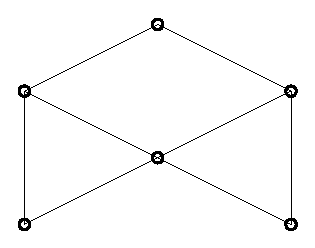
\includegraphics{fig/celula_correta.eps}
    \caption[Elemento conforme]{Elemento conforme}
    \label{fig:celula_correta}
\end{figure}


\begin{figure}
    \centering
    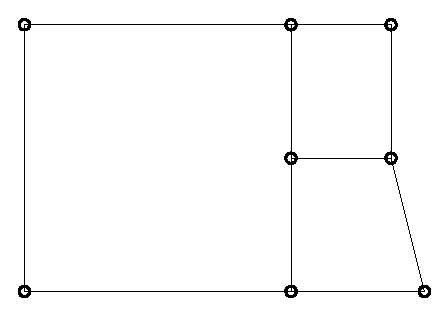
\includegraphics{fig/celula_errada.eps}
    \caption[Elemento não conforme]{Elemento não conforme}
    \label{fig:celula_errada}
\end{figure}

O objetivo da geração de malhas é criar elementos que se conformam com o formato e com a geometria do problema e obedeçam a restrições em seu tamanho e formato.

Nas malhas, tem-se que as fronteiras existem de modo a se poder aplicar as condições de contorno para a equação diferencial parcial e para permitir a descontinuidade nas propriedades físicas, como por exemplo diferenças na condutividade de calor. Uma fronteira, deve ser representada pela união de duas faces na malha. Elementos não podem cruzar essa fronteira, e no local onde dois materiais se encontram, suas malhas devem ter faces equivalentes. Esse requisito faz com que a geração de malhas seja mais difícil se o domínio possuir ângulos pequenos.

\subsection{Elementos desejados}
Um bom elemento de malha deve seguir várias restrições de modo a produzir um bom resultado numérico. Essas restrições possuem várias origens. Primeiramente, ângulos grandes causam um grande erro de interpolação. Segundamente, ângulos pequenos 


A triangulação de Delaunay para um conjunto de pontos discretos P em um plano é uma triangularização que faz com que nenhum ponto em P esteja dentro do circuncirculo de qualquer triangulo formado pelo algoritmo.

A triangularização de Delaunay maximiza o menor angulo de todos os ângulos criados pela triangularização. O nome desse método vem de Boris Delaunay em seu trabalho no tópico em 1934.

Para um conjunto de pontos em uma mesma linha, não existe triangularização de Delaunay (a noção de triangulo nesse caso é degenerada). Para quatro ou mais pontos em um mesmo círculo (por exemplo os vértices de um retânculo) a triangularização não é única, pois cada um dos possíveis triangulos que dividem o quadrado satisfazem a "condição de Delaunay", ie., a confição de que os circuncírculos de todos os triangulos tenham interiores vazios.